\documentclass[tikz,border=5pt]{standalone}
\usepackage{amsmath,amssymb,centernot}
\begin{document}
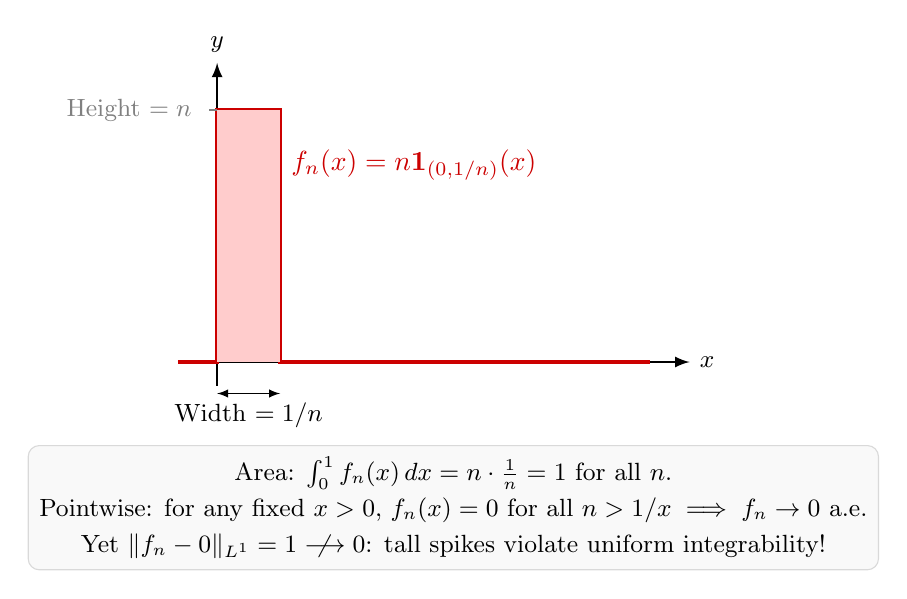
\begin{tikzpicture}[>=latex, font=\small]
  \draw[->, thick] (-0.5, 0) -- (6.0, 0) node[right] {$x$};
  \draw[->, thick] (0, -0.3) -- (0, 3.8) node[above] {$y$};

  % Spike
  \draw[very thick, red!80!black] (-0.5, 0) -- (0, 0) -- (0, 3.2) -- (0.8, 3.2) -- (0.8, 0) -- (5.5, 0);
  \fill[red!20] (0, 0) rectangle (0.8, 3.2);

  \draw[dashed, gray] (0, 3.2) -- (-0.2, 3.2) node[left] {Height $= n$};
  \draw[<->] (0, -0.4) -- (0.8, -0.4) node[midway, below] {Width $= 1/n$};

  \node[font=\bfseries, red!80!black] at (2.5, 2.5) {$f_n(x) = n \mathbf{1}_{(0, 1/n)}(x)$};

  \node[align=center, fill=gray!5, draw=gray!30, rounded corners, inner sep=4pt] at (3.0, -1.85)
    {Area: $\int_0^1 f_n(x)\,dx = n \cdot \frac{1}{n} = 1$ for all $n$.\\[2pt]
     Pointwise: for any fixed $x > 0$, $f_n(x) = 0$ for all $n > 1/x \implies f_n \to 0$ a.e.\\[2pt]
     Yet $\|f_n - 0\|_{L^1} = 1 \centernot\longrightarrow 0$: tall spikes violate uniform integrability!};
\end{tikzpicture}
\end{document}
